\documentclass[]{article}
\usepackage{lmodern}
\usepackage{amssymb,amsmath}
\usepackage{ifxetex,ifluatex}
\usepackage{fixltx2e} % provides \textsubscript
\ifnum 0\ifxetex 1\fi\ifluatex 1\fi=0 % if pdftex
  \usepackage[T1]{fontenc}
  \usepackage[utf8]{inputenc}
\else % if luatex or xelatex
  \ifxetex
    \usepackage{mathspec}
  \else
    \usepackage{fontspec}
  \fi
  \defaultfontfeatures{Ligatures=TeX,Scale=MatchLowercase}
\fi
% use upquote if available, for straight quotes in verbatim environments
\IfFileExists{upquote.sty}{\usepackage{upquote}}{}
% use microtype if available
\IfFileExists{microtype.sty}{%
\usepackage{microtype}
\UseMicrotypeSet[protrusion]{basicmath} % disable protrusion for tt fonts
}{}
\usepackage[margin=1in]{geometry}
\usepackage{hyperref}
\hypersetup{unicode=true,
            pdfborder={0 0 0},
            breaklinks=true}
\urlstyle{same}  % don't use monospace font for urls
\usepackage{color}
\usepackage{fancyvrb}
\newcommand{\VerbBar}{|}
\newcommand{\VERB}{\Verb[commandchars=\\\{\}]}
\DefineVerbatimEnvironment{Highlighting}{Verbatim}{commandchars=\\\{\}}
% Add ',fontsize=\small' for more characters per line
\usepackage{framed}
\definecolor{shadecolor}{RGB}{248,248,248}
\newenvironment{Shaded}{\begin{snugshade}}{\end{snugshade}}
\newcommand{\AlertTok}[1]{\textcolor[rgb]{0.94,0.16,0.16}{#1}}
\newcommand{\AnnotationTok}[1]{\textcolor[rgb]{0.56,0.35,0.01}{\textbf{\textit{#1}}}}
\newcommand{\AttributeTok}[1]{\textcolor[rgb]{0.77,0.63,0.00}{#1}}
\newcommand{\BaseNTok}[1]{\textcolor[rgb]{0.00,0.00,0.81}{#1}}
\newcommand{\BuiltInTok}[1]{#1}
\newcommand{\CharTok}[1]{\textcolor[rgb]{0.31,0.60,0.02}{#1}}
\newcommand{\CommentTok}[1]{\textcolor[rgb]{0.56,0.35,0.01}{\textit{#1}}}
\newcommand{\CommentVarTok}[1]{\textcolor[rgb]{0.56,0.35,0.01}{\textbf{\textit{#1}}}}
\newcommand{\ConstantTok}[1]{\textcolor[rgb]{0.00,0.00,0.00}{#1}}
\newcommand{\ControlFlowTok}[1]{\textcolor[rgb]{0.13,0.29,0.53}{\textbf{#1}}}
\newcommand{\DataTypeTok}[1]{\textcolor[rgb]{0.13,0.29,0.53}{#1}}
\newcommand{\DecValTok}[1]{\textcolor[rgb]{0.00,0.00,0.81}{#1}}
\newcommand{\DocumentationTok}[1]{\textcolor[rgb]{0.56,0.35,0.01}{\textbf{\textit{#1}}}}
\newcommand{\ErrorTok}[1]{\textcolor[rgb]{0.64,0.00,0.00}{\textbf{#1}}}
\newcommand{\ExtensionTok}[1]{#1}
\newcommand{\FloatTok}[1]{\textcolor[rgb]{0.00,0.00,0.81}{#1}}
\newcommand{\FunctionTok}[1]{\textcolor[rgb]{0.00,0.00,0.00}{#1}}
\newcommand{\ImportTok}[1]{#1}
\newcommand{\InformationTok}[1]{\textcolor[rgb]{0.56,0.35,0.01}{\textbf{\textit{#1}}}}
\newcommand{\KeywordTok}[1]{\textcolor[rgb]{0.13,0.29,0.53}{\textbf{#1}}}
\newcommand{\NormalTok}[1]{#1}
\newcommand{\OperatorTok}[1]{\textcolor[rgb]{0.81,0.36,0.00}{\textbf{#1}}}
\newcommand{\OtherTok}[1]{\textcolor[rgb]{0.56,0.35,0.01}{#1}}
\newcommand{\PreprocessorTok}[1]{\textcolor[rgb]{0.56,0.35,0.01}{\textit{#1}}}
\newcommand{\RegionMarkerTok}[1]{#1}
\newcommand{\SpecialCharTok}[1]{\textcolor[rgb]{0.00,0.00,0.00}{#1}}
\newcommand{\SpecialStringTok}[1]{\textcolor[rgb]{0.31,0.60,0.02}{#1}}
\newcommand{\StringTok}[1]{\textcolor[rgb]{0.31,0.60,0.02}{#1}}
\newcommand{\VariableTok}[1]{\textcolor[rgb]{0.00,0.00,0.00}{#1}}
\newcommand{\VerbatimStringTok}[1]{\textcolor[rgb]{0.31,0.60,0.02}{#1}}
\newcommand{\WarningTok}[1]{\textcolor[rgb]{0.56,0.35,0.01}{\textbf{\textit{#1}}}}
\usepackage{longtable,booktabs}
\usepackage{graphicx,grffile}
\makeatletter
\def\maxwidth{\ifdim\Gin@nat@width>\linewidth\linewidth\else\Gin@nat@width\fi}
\def\maxheight{\ifdim\Gin@nat@height>\textheight\textheight\else\Gin@nat@height\fi}
\makeatother
% Scale images if necessary, so that they will not overflow the page
% margins by default, and it is still possible to overwrite the defaults
% using explicit options in \includegraphics[width, height, ...]{}
\setkeys{Gin}{width=\maxwidth,height=\maxheight,keepaspectratio}
\IfFileExists{parskip.sty}{%
\usepackage{parskip}
}{% else
\setlength{\parindent}{0pt}
\setlength{\parskip}{6pt plus 2pt minus 1pt}
}
\setlength{\emergencystretch}{3em}  % prevent overfull lines
\providecommand{\tightlist}{%
  \setlength{\itemsep}{0pt}\setlength{\parskip}{0pt}}
\setcounter{secnumdepth}{0}
% Redefines (sub)paragraphs to behave more like sections
\ifx\paragraph\undefined\else
\let\oldparagraph\paragraph
\renewcommand{\paragraph}[1]{\oldparagraph{#1}\mbox{}}
\fi
\ifx\subparagraph\undefined\else
\let\oldsubparagraph\subparagraph
\renewcommand{\subparagraph}[1]{\oldsubparagraph{#1}\mbox{}}
\fi

%%% Use protect on footnotes to avoid problems with footnotes in titles
\let\rmarkdownfootnote\footnote%
\def\footnote{\protect\rmarkdownfootnote}

%%% Change title format to be more compact
\usepackage{titling}

% Create subtitle command for use in maketitle
\providecommand{\subtitle}[1]{
  \posttitle{
    \begin{center}\large#1\end{center}
    }
}

\setlength{\droptitle}{-2em}

  \title{}
    \pretitle{\vspace{\droptitle}}
  \posttitle{}
    \author{}
    \preauthor{}\postauthor{}
    \date{}
    \predate{}\postdate{}
  

\begin{document}

class: center, middle

\hypertarget{data-analysis-in-r}{%
\section{Data Analysis in R}\label{data-analysis-in-r}}

Adam Rawles

\begin{center}\rule{0.5\linewidth}{\linethickness}\end{center}

\hypertarget{recap}{%
\subsection{Recap}\label{recap}}

--

\begin{itemize}
\tightlist
\item
  What is R and RStudio?
\end{itemize}

--

\begin{itemize}
\tightlist
\item
  Basic arithmetic operators
\end{itemize}

--

\begin{itemize}
\tightlist
\item
  Variable assigment
\end{itemize}

--

\begin{itemize}
\tightlist
\item
  Data types
\end{itemize}

--

\begin{itemize}
\tightlist
\item
  Data structures (including subsetting)
\end{itemize}

--

\begin{itemize}
\tightlist
\item
  Functions
\end{itemize}

\begin{center}\rule{0.5\linewidth}{\linethickness}\end{center}

\hypertarget{overview}{%
\subsection{Overview}\label{overview}}

--

\begin{itemize}
\tightlist
\item
  Installing packages
\end{itemize}

--

\begin{itemize}
\tightlist
\item
  Loading data
\end{itemize}

--

\begin{itemize}
\tightlist
\item
  Cleaning data
\end{itemize}

--

\begin{itemize}
\tightlist
\item
  Summary statistics
\end{itemize}

--

\begin{itemize}
\tightlist
\item
  Graphs and plots
\end{itemize}

\begin{center}\rule{0.5\linewidth}{\linethickness}\end{center}

\hypertarget{installing-packages}{%
\subsection{Installing packages}\label{installing-packages}}

\begin{itemize}
\tightlist
\item
  Packages provide extra functions and/or data to R (for example, the
  \texttt{stringr} package provides functions to help with text
  cleaning)
\end{itemize}

--

\begin{itemize}
\tightlist
\item
  Installing packages with RStudio is easy to do
\end{itemize}

--

\begin{itemize}
\tightlist
\item
  RStudio has a built-in interface for installing packages\ldots{}
\item
  Or, you can use the R function \texttt{install.packages()}, and
  provide the name of the package(s) you want to install to the function
\end{itemize}

--

\begin{Shaded}
\begin{Highlighting}[]
\KeywordTok{install.packages}\NormalTok{(}\StringTok{"ggplot2"}\NormalTok{)}
\KeywordTok{install.packages}\NormalTok{(}\KeywordTok{c}\NormalTok{(}\StringTok{"ggplot2"}\NormalTok{, }\StringTok{"dplyr"}\NormalTok{))}
\end{Highlighting}
\end{Shaded}

--

\begin{itemize}
\tightlist
\item
  Packages must be loaded before they are available, via the
  \texttt{library()} function
\end{itemize}

--

\begin{Shaded}
\begin{Highlighting}[]
\KeywordTok{library}\NormalTok{(ggplot2)}
\end{Highlighting}
\end{Shaded}

\begin{itemize}
\tightlist
\item
  Note: if you close RStudio, you'll need to reload your packages.
\item
  Think of installing the package being like installing a program, and
  the \texttt{library()} call as like opening it - you wouldn't open a
  program without installing it and you wouldn't use it without opening
  it!
\end{itemize}

\begin{center}\rule{0.5\linewidth}{\linethickness}\end{center}

\hypertarget{using-packages}{%
\subsection{Using packages}\label{using-packages}}

\begin{itemize}
\tightlist
\item
  If you've loaded a pacakge via \texttt{library()}, then you don't need
  to do anything else before you use it.
\end{itemize}

--

\begin{itemize}
\tightlist
\item
  However, when using a non-base R function or if you haven't loaded the
  package, it's always a good idea to make it explicit what package it
  came from.
\end{itemize}

--

\begin{itemize}
\tightlist
\item
  We do that using \texttt{::}
\end{itemize}

--

\begin{Shaded}
\begin{Highlighting}[]
\NormalTok{ggplot2}\OperatorTok{::}\KeywordTok{ggplot}\NormalTok{()}
\end{Highlighting}
\end{Shaded}

--

\begin{itemize}
\tightlist
\item
  This will mean that anyone reading your code will know exactly what
  package a function came from
\end{itemize}

--

\begin{itemize}
\tightlist
\item
  It'll also ensure that you're using the function you mean to in the
  event that two packages have functions with the same name
\end{itemize}

\begin{center}\rule{0.5\linewidth}{\linethickness}\end{center}

\hypertarget{loading-data}{%
\subsection{Loading data}\label{loading-data}}

--

\begin{itemize}
\tightlist
\item
  Data can be loaded into R in many formats
\end{itemize}

--

\begin{itemize}
\tightlist
\item
  The easiest of which are .xlsx or .csv files
\end{itemize}

--

\begin{itemize}
\tightlist
\item
  These can be loaded into R two different ways
\end{itemize}

--

\begin{itemize}
\tightlist
\item
  The first is by using the \texttt{read.csv()}/\texttt{read.xlsx()}
  functions
\end{itemize}

--

\begin{quote}
\begin{itemize}
\tightlist
\item
  The \texttt{read.csv()} function takes a string of the file's path as
  it's only required input argument
\end{itemize}
\end{quote}

--

\begin{quote}
\begin{quote}
\begin{itemize}
\tightlist
\item
  But there are a number of optional arguments (e.g.~\texttt{header},
  \texttt{stringsAsFactor},\ldots)
\end{itemize}
\end{quote}
\end{quote}

--

\begin{quote}
\begin{itemize}
\tightlist
\item
  The \texttt{read.xlsx()} function requires both a path, and the index
  of the sheet you want from the workbook
\end{itemize}
\end{quote}

\begin{center}\rule{0.5\linewidth}{\linethickness}\end{center}

\hypertarget{loading-data-1}{%
\subsection{Loading data}\label{loading-data-1}}

\begin{itemize}
\tightlist
\item
  The second is to use RStudio's built in ``Import Dataset'' interface
\end{itemize}

--

\begin{itemize}
\tightlist
\item
  This interface essentially just acts as a wrapper to the
  \texttt{read.csv()/xlsx()} functions
\item
  You'll see that when you run it, the code to import the data is run in
  the console
\end{itemize}

\begin{center}\rule{0.5\linewidth}{\linethickness}\end{center}

\hypertarget{loading-data---example}{%
\subsection{Loading data - example}\label{loading-data---example}}

\begin{center}\rule{0.5\linewidth}{\linethickness}\end{center}

\hypertarget{loading-data---example-1}{%
\subsection{Loading data - example}\label{loading-data---example-1}}

\begin{Shaded}
\begin{Highlighting}[]
\NormalTok{test_data <-}\StringTok{ }\KeywordTok{read.csv}\NormalTok{(}\StringTok{"test_data.csv"}\NormalTok{,}
                      \DataTypeTok{header =} \OtherTok{TRUE}\NormalTok{,}
                      \DataTypeTok{stringsAsFactors =} \OtherTok{TRUE}\NormalTok{)}

\KeywordTok{head}\NormalTok{(test_data, }\DataTypeTok{n =} \DecValTok{2}\NormalTok{)}
\end{Highlighting}
\end{Shaded}

\begin{verbatim}
##   Firm LeadDivision Income Employees ReturnDate
## 1    X      Banking   1000        50 01/01/2018
## 2    B    Fiduciary   2000        60 01/06/2018
\end{verbatim}

\begin{center}\rule{0.5\linewidth}{\linethickness}\end{center}

\hypertarget{loading-data---exercise}{%
\subsection{Loading data - exercise}\label{loading-data---exercise}}

--

\begin{itemize}
\tightlist
\item
  Using RStudio's ``Import Dataset'' or the \texttt{read.csv()}
  function, load the test\_data dataset
\end{itemize}

\begin{center}\rule{0.5\linewidth}{\linethickness}\end{center}

\hypertarget{data-cleaning}{%
\subsection{Data cleaning}\label{data-cleaning}}

--

\begin{itemize}
\tightlist
\item
  After the data is loaded into R, we need to make sure that each column
  is in the correct format (e.g.~character, factor, numeric, etc.)
\end{itemize}

--

\begin{itemize}
\tightlist
\item
  This can be done two different ways:
\end{itemize}

\begin{longtable}[]{@{}r@{}}
\toprule
\endhead
\begin{minipage}[t]{0.04\columnwidth}\raggedleft
- You can either click on the dataframe in the Environment pane, which
will open the dataframe in the Source pane\strut
\end{minipage}\tabularnewline
\bottomrule
\end{longtable}

\begin{quote}
\begin{itemize}
\tightlist
\item
  From here, you can hover over the column headers to see what type the
  data is stored as
\item
  Or, you can use the is.xxxxx functions to check from the console.
\end{itemize}
\end{quote}

--

\begin{quote}
\begin{verbatim}
 - To do this, you choose the appropriate function for the type you want (e.g. `is.numeric()`), and include the column you want to check as an argument...
\end{verbatim}
\end{quote}

\begin{center}\rule{0.5\linewidth}{\linethickness}\end{center}

\hypertarget{data-cleaning-1}{%
\subsection{Data cleaning}\label{data-cleaning-1}}

\begin{Shaded}
\begin{Highlighting}[]
\KeywordTok{is.numeric}\NormalTok{(test_data}\OperatorTok{$}\NormalTok{Income)}
\end{Highlighting}
\end{Shaded}

\begin{verbatim}
## [1] TRUE
\end{verbatim}

\begin{Shaded}
\begin{Highlighting}[]
\CommentTok{## we could also do is.numeric(test_data[,1]) as per our last session on subsetting}

\KeywordTok{is.numeric}\NormalTok{(test_data}\OperatorTok{$}\NormalTok{LeadDivsion)}
\end{Highlighting}
\end{Shaded}

\begin{verbatim}
## [1] FALSE
\end{verbatim}

\begin{Shaded}
\begin{Highlighting}[]
\KeywordTok{is.factor}\NormalTok{(test_data}\OperatorTok{$}\NormalTok{LeadDivision)}
\end{Highlighting}
\end{Shaded}

\begin{verbatim}
## [1] TRUE
\end{verbatim}

\begin{center}\rule{0.5\linewidth}{\linethickness}\end{center}

\hypertarget{data-cleaning-2}{%
\subsection{Data cleaning}\label{data-cleaning-2}}

\begin{itemize}
\tightlist
\item
  If you want to get the type of a column without comparing it to other
  types, you use the \texttt{is()} function
\end{itemize}

--

\begin{itemize}
\tightlist
\item
  The first value returned from this function will tell you the data
  type of the column
\end{itemize}

\begin{Shaded}
\begin{Highlighting}[]
\KeywordTok{is}\NormalTok{(test_data}\OperatorTok{$}\NormalTok{Firm)}
\end{Highlighting}
\end{Shaded}

\begin{verbatim}
## [1] "factor"              "integer"             "oldClass"           
## [4] "double"              "numeric"             "vector"             
## [7] "data.frameRowLabels"
\end{verbatim}

\begin{Shaded}
\begin{Highlighting}[]
\KeywordTok{is}\NormalTok{(test_data}\OperatorTok{$}\NormalTok{Employees)}
\end{Highlighting}
\end{Shaded}

\begin{verbatim}
## [1] "integer"             "double"              "numeric"            
## [4] "vector"              "data.frameRowLabels"
\end{verbatim}

\begin{center}\rule{0.5\linewidth}{\linethickness}\end{center}

\hypertarget{data-cleaning-3}{%
\subsection{Data cleaning}\label{data-cleaning-3}}

\begin{itemize}
\tightlist
\item
  If a column does not have the correct type, we can easily coerce the
  values into the type that we want
\end{itemize}

--

\begin{itemize}
\tightlist
\item
  The exact method is different depending on what you are converting
  from and to
\end{itemize}

--

\begin{itemize}
\tightlist
\item
  Generally speaking however, the method for converting a column type
  is:
\end{itemize}

\begin{Shaded}
\begin{Highlighting}[]
\NormalTok{dataframe}\OperatorTok{$}\NormalTok{column <-}\StringTok{ }\KeywordTok{as.xxxxx}\NormalTok{(dataframe}\OperatorTok{$}\NormalTok{column)}
\end{Highlighting}
\end{Shaded}

\begin{center}\rule{0.5\linewidth}{\linethickness}\end{center}

\hypertarget{data-cleaning---exercise}{%
\subsection{Data cleaning - exercise}\label{data-cleaning---exercise}}

--

\begin{itemize}
\tightlist
\item
  Convert the the Firm column from a factor to a character, and check
  your conversion worked
\end{itemize}

\begin{center}\rule{0.5\linewidth}{\linethickness}\end{center}

\hypertarget{date-cleaning---answer}{%
\subsection{Date cleaning - answer}\label{date-cleaning---answer}}

\begin{Shaded}
\begin{Highlighting}[]
\NormalTok{test_data}\OperatorTok{$}\NormalTok{Firm <-}\StringTok{ }\KeywordTok{as.character}\NormalTok{(test_data}\OperatorTok{$}\NormalTok{Firm)}

\KeywordTok{is.character}\NormalTok{(test_data}\OperatorTok{$}\NormalTok{Firm)}
\end{Highlighting}
\end{Shaded}

\begin{verbatim}
## [1] TRUE
\end{verbatim}

\begin{center}\rule{0.5\linewidth}{\linethickness}\end{center}

\hypertarget{data-cleaning-4}{%
\subsection{Data cleaning}\label{data-cleaning-4}}

\begin{itemize}
\tightlist
\item
  This method works well for:
\end{itemize}

--

\begin{itemize}
\tightlist
\item
  Numeric/integer to character
\end{itemize}

--

\begin{itemize}
\tightlist
\item
  Character to numeric/integer
\end{itemize}

--

\begin{itemize}
\tightlist
\item
  Integer to numeric
\end{itemize}

--

\begin{itemize}
\tightlist
\item
  Numeric to integer
\end{itemize}

--

\begin{itemize}
\tightlist
\item
  Character to factor
\end{itemize}

--

\begin{itemize}
\tightlist
\item
  Factor to character
\end{itemize}

--

\begin{itemize}
\tightlist
\item
  Numeric to factor
\end{itemize}

--

\begin{itemize}
\tightlist
\item
  For factor to numeric, there's an extra step:
\end{itemize}

--

\begin{itemize}
\tightlist
\item
  Before the factors levels can be converted, they need to be converted
  to characters first:
\end{itemize}

\begin{Shaded}
\begin{Highlighting}[]
\NormalTok{dataframe}\OperatorTok{$}\NormalTok{column <-}\StringTok{ }\KeywordTok{as.numeric}\NormalTok{(}\KeywordTok{as.character}\NormalTok{(dataframe}\OperatorTok{$}\NormalTok{column))}
\end{Highlighting}
\end{Shaded}

\begin{center}\rule{0.5\linewidth}{\linethickness}\end{center}

\hypertarget{data-cleaning---dates}{%
\subsection{Data cleaning - dates}\label{data-cleaning---dates}}

\begin{itemize}
\tightlist
\item
  Dates in R can be tricky
\end{itemize}

--

\begin{itemize}
\item ~
  \hypertarget{r-will-not-import-date-values-in-as-dates-unless-you-specify-that-it-should}{%
  \subsection{R will not import date values in as dates unless you
  specify that it
  should}\label{r-will-not-import-date-values-in-as-dates-unless-you-specify-that-it-should}}

  \begin{itemize}
  \tightlist
  \item
    But RStudio's ``Import Dataset'' feature can be handy here\ldots{}
  \end{itemize}
\end{itemize}

--

\begin{itemize}
\tightlist
\item
  If you don't, R will import them as characters (which means they'll be
  converted to factors unless you specify
  \texttt{stringsAsFactors\ =\ FALSE})
\end{itemize}

--

\begin{itemize}
\tightlist
\item
  To convert a character to a date, use the \texttt{as.Date()}
  function\ldots{}
\end{itemize}

\begin{center}\rule{0.5\linewidth}{\linethickness}\end{center}

\hypertarget{data-cleaning---dates-example}{%
\subsection{Data cleaning - dates
(example)}\label{data-cleaning---dates-example}}

\begin{Shaded}
\begin{Highlighting}[]
\NormalTok{datetest <-}\StringTok{ "12/12/2018"}
\NormalTok{datetest <-}\StringTok{ }\KeywordTok{as.Date}\NormalTok{(datetest, }\DataTypeTok{format =} \StringTok{"%d/%m/%Y"}\NormalTok{)}
\KeywordTok{is}\NormalTok{(datetest)}
\end{Highlighting}
\end{Shaded}

\begin{verbatim}
## [1] "Date"     "oldClass"
\end{verbatim}

--

\begin{itemize}
\tightlist
\item
  To convert from a factor to a date, first convert to a
  character\ldots{}
\end{itemize}

\begin{center}\rule{0.5\linewidth}{\linethickness}\end{center}

\hypertarget{data-cleaning---dates-exercise}{%
\subsection{Data cleaning - dates
(exercise)}\label{data-cleaning---dates-exercise}}

\begin{itemize}
\tightlist
\item
  Our \texttt{test\_data\$ReturnDate} column is currently a factor,
  convert it to date
\end{itemize}

--

\begin{itemize}
\tightlist
\item
  Remember to convert the column to character first!
\end{itemize}

\begin{center}\rule{0.5\linewidth}{\linethickness}\end{center}

\hypertarget{data-cleaning---datesanswer}{%
\subsection{Data cleaning -
dates(answer)}\label{data-cleaning---datesanswer}}

\begin{Shaded}
\begin{Highlighting}[]
\NormalTok{test_data}\OperatorTok{$}\NormalTok{ReturnDate <-}\StringTok{ }\KeywordTok{as.character}\NormalTok{(test_data}\OperatorTok{$}\NormalTok{ReturnDate)}
\NormalTok{test_data}\OperatorTok{$}\NormalTok{ReturnDate <-}\StringTok{ }\KeywordTok{as.Date}\NormalTok{(test_data}\OperatorTok{$}\NormalTok{ReturnDate,}
                                \DataTypeTok{format =} \StringTok{"%d/%m/%Y"}\NormalTok{)}
\end{Highlighting}
\end{Shaded}

\begin{Shaded}
\begin{Highlighting}[]
\NormalTok{test_data}\OperatorTok{$}\NormalTok{ReturnDate <-}\StringTok{ }\KeywordTok{as.Date}\NormalTok{(}\KeywordTok{as.character}\NormalTok{(test_data}\OperatorTok{$}\NormalTok{ReturnDate),}
                                \DataTypeTok{format =} \StringTok{"%d/%m/%Y"}\NormalTok{)}
\end{Highlighting}
\end{Shaded}

\begin{center}\rule{0.5\linewidth}{\linethickness}\end{center}

\hypertarget{data-cleaning---dates-1}{%
\subsection{Data cleaning - dates}\label{data-cleaning---dates-1}}

\begin{itemize}
\tightlist
\item
  Dates can also come in numeric form, calculated as the number of days
  from a particular origin
\end{itemize}

--

\begin{itemize}
\tightlist
\item
  For example, a numeric value of 1, with an origin of 12/12/2018 would
  correspond to a date value of 13/12/2018
\end{itemize}

--

\begin{itemize}
\tightlist
\item
  If your date values are in numeric format, you need to specify the
  origin in the \texttt{as.Date()} function\ldots{}
\end{itemize}

\begin{center}\rule{0.5\linewidth}{\linethickness}\end{center}

\hypertarget{data-cleaning---dates-example-1}{%
\subsection{Data cleaning - dates
(example)}\label{data-cleaning---dates-example-1}}

\begin{Shaded}
\begin{Highlighting}[]
\NormalTok{datetest <-}\StringTok{ }\DecValTok{17940}
\NormalTok{datetest <-}\StringTok{ }\KeywordTok{as.Date}\NormalTok{(datetest,}
                    \DataTypeTok{origin =} \KeywordTok{as.Date}\NormalTok{(}\StringTok{"01/01/1970"}\NormalTok{,}
                                     \DataTypeTok{format =} \StringTok{"%d/%m/%Y"}\NormalTok{))}
\NormalTok{datetest}
\end{Highlighting}
\end{Shaded}

\begin{verbatim}
## [1] "2019-02-13"
\end{verbatim}

\begin{center}\rule{0.5\linewidth}{\linethickness}\end{center}

\hypertarget{data-cleaning---dates-2}{%
\subsection{Data cleaning - dates}\label{data-cleaning---dates-2}}

\begin{itemize}
\tightlist
\item
  With dates, you'll often need to specify the format (format codes can
  be found online and are included in your help sheet)
\end{itemize}

--

\begin{itemize}
\tightlist
\item
  There's no \texttt{is.Date()} function in base R
\end{itemize}

--

\begin{itemize}
\tightlist
\item
  So to check whether a value is a date, use \texttt{is()}
\end{itemize}

\begin{center}\rule{0.5\linewidth}{\linethickness}\end{center}

\hypertarget{data-cleaning---conclusion}{%
\subsection{Data cleaning -
conclusion}\label{data-cleaning---conclusion}}

\begin{itemize}
\tightlist
\item
  To find out the type of a column, use the \texttt{is()} function
\end{itemize}

--

\begin{itemize}
\tightlist
\item
  Otherwise, you can (usually) test if a column is a specific type via
  the is.xxxxx functions
\end{itemize}

--

\begin{itemize}
\tightlist
\item
  Converting between datatypes (except from numeric -\textgreater{}
  factor) is easy with the as.xxxxx functions
\end{itemize}

--

\begin{itemize}
\tightlist
\item
  When converting numbers to factors, convert them to characters first
\end{itemize}

--

\begin{itemize}
\tightlist
\item
  When converting from characters or numeric to dates,
  \texttt{as.Date()} requires ``format'' or ``origin'' parameters
  respectively
\end{itemize}

\begin{center}\rule{0.5\linewidth}{\linethickness}\end{center}

\hypertarget{summary-statistics}{%
\subsection{Summary statistics}\label{summary-statistics}}

\begin{itemize}
\tightlist
\item
  Before doing any in-depth analysis, it's always a good idea to get
  some descriptive statistics from your data
\end{itemize}

--

\begin{itemize}
\tightlist
\item
  This includes the mean, the median, the standard deviation, and the
  interquartile range, but the statistics you use will depend on your
  data
\end{itemize}

--

\begin{itemize}
\tightlist
\item
  Getting these values for each column is easy using the built-in
  functions R provides:
\end{itemize}

\begin{Shaded}
\begin{Highlighting}[]
\KeywordTok{mean}\NormalTok{()}
\KeywordTok{median}\NormalTok{()}
\KeywordTok{sd}\NormalTok{()}
\KeywordTok{quantile}\NormalTok{()}
\end{Highlighting}
\end{Shaded}

\begin{center}\rule{0.5\linewidth}{\linethickness}\end{center}

\hypertarget{summary-statistics---exercise}{%
\subsection{Summary statistics -
exercise}\label{summary-statistics---exercise}}

\begin{itemize}
\tightlist
\item
  Find the mean, median, standard deviation, and quantiles for our meter
  reading column
\end{itemize}

\begin{center}\rule{0.5\linewidth}{\linethickness}\end{center}

\hypertarget{summary-statistics---answers}{%
\subsection{Summary statistics -
answers}\label{summary-statistics---answers}}

\begin{Shaded}
\begin{Highlighting}[]
\KeywordTok{mean}\NormalTok{(test_data}\OperatorTok{$}\NormalTok{Income)}
\end{Highlighting}
\end{Shaded}

\begin{verbatim}
## [1] 4434.174
\end{verbatim}

\begin{Shaded}
\begin{Highlighting}[]
\KeywordTok{median}\NormalTok{(test_data}\OperatorTok{$}\NormalTok{Income)}
\end{Highlighting}
\end{Shaded}

\begin{verbatim}
## [1] 3528
\end{verbatim}

\begin{Shaded}
\begin{Highlighting}[]
\KeywordTok{sd}\NormalTok{(test_data}\OperatorTok{$}\NormalTok{Income)}
\end{Highlighting}
\end{Shaded}

\begin{verbatim}
## [1] 2574.724
\end{verbatim}

\begin{Shaded}
\begin{Highlighting}[]
\KeywordTok{quantile}\NormalTok{(test_data}\OperatorTok{$}\NormalTok{Income)}
\end{Highlighting}
\end{Shaded}

\begin{verbatim}
##      0%     25%     50%     75%    100% 
##  1000.0  2930.5  3528.0  5850.5 10000.0
\end{verbatim}

\begin{center}\rule{0.5\linewidth}{\linethickness}\end{center}

\hypertarget{summary-statistics-1}{%
\subsection{Summary statistics}\label{summary-statistics-1}}

\begin{itemize}
\tightlist
\item
  More often than not however, you'll want summary statistics for more
  than one column, or maybe broken down by group
\end{itemize}

--

\begin{itemize}
\tightlist
\item
  R includes a function that will give you summary statistics for each
  column (the \texttt{summary()} function):
\end{itemize}

\begin{Shaded}
\begin{Highlighting}[]
\KeywordTok{summary}\NormalTok{(test_data)}
\end{Highlighting}
\end{Shaded}

\begin{verbatim}
##      Firm               LeadDivision     Income        Employees     
##  Length:23          Banking   :10    Min.   : 1000   Min.   : 40.00  
##  Class :character   Fiduciary : 5    1st Qu.: 2930   1st Qu.: 48.00  
##  Mode  :character   Insurance : 4    Median : 3528   Median : 59.00  
##                     Investment: 4    Mean   : 4434   Mean   : 65.22  
##                                      3rd Qu.: 5850   3rd Qu.: 67.50  
##                                      Max.   :10000   Max.   :150.00  
##    ReturnDate        
##  Min.   :2018-01-01  
##  1st Qu.:2018-01-01  
##  Median :2018-06-01  
##  Mean   :2018-05-03  
##  3rd Qu.:2018-06-01  
##  Max.   :2019-01-01
\end{verbatim}

\begin{center}\rule{0.5\linewidth}{\linethickness}\end{center}

\hypertarget{summary-statistics-by-group}{%
\subsection{Summary statistics by
group}\label{summary-statistics-by-group}}

\begin{itemize}
\tightlist
\item
  Summary statistics by group are a little bit more complicated as they
  require us to ``apply'' the function for each group
\end{itemize}

--

\begin{itemize}
\tightlist
\item
  To do that, we use the \texttt{tapply()} function. This will take the
  test\_data dataset, split it according to the grouping we give, and
  then use whatever summary function we provide
\end{itemize}

--

\begin{Shaded}
\begin{Highlighting}[]
\KeywordTok{tapply}\NormalTok{(test_data}\OperatorTok{$}\NormalTok{Income, test_data}\OperatorTok{$}\NormalTok{LeadDivision, sd)}
\end{Highlighting}
\end{Shaded}

\begin{verbatim}
##    Banking  Fiduciary  Insurance Investment 
##  3077.5284  3321.5053  1876.4645   870.7002
\end{verbatim}

--

\begin{itemize}
\item ~
  \hypertarget{so-here-we-provide-the-income-column-say-to-split-it-up-by-lead-division-and-apply-the-sd-function}{%
  \subsection{\texorpdfstring{So here we provide the Income column, say
  to split it up by Lead Division, and apply the \texttt{sd()}
  function}{So here we provide the Income column, say to split it up by Lead Division, and apply the sd() function}}\label{so-here-we-provide-the-income-column-say-to-split-it-up-by-lead-division-and-apply-the-sd-function}}
\end{itemize}

\hypertarget{summary-statistics-by-group---exercise}{%
\subsection{Summary statistics by group -
exercise}\label{summary-statistics-by-group---exercise}}

\begin{itemize}
\tightlist
\item
  Produce the mean income for each division
\end{itemize}

\begin{center}\rule{0.5\linewidth}{\linethickness}\end{center}

\hypertarget{summary-statistics-by-group---answer}{%
\subsection{Summary statistics by group -
answer}\label{summary-statistics-by-group---answer}}

\begin{Shaded}
\begin{Highlighting}[]
\KeywordTok{tapply}\NormalTok{(test_data}\OperatorTok{$}\NormalTok{Income, test_data}\OperatorTok{$}\NormalTok{LeadDivision, mean)}
\end{Highlighting}
\end{Shaded}

\begin{verbatim}
##    Banking  Fiduciary  Insurance Investment 
##    4356.50    5124.00    4294.50    3905.75
\end{verbatim}

\begin{center}\rule{0.5\linewidth}{\linethickness}\end{center}

\hypertarget{summary-statistics---conclusion}{%
\subsection{Summary statistics -
conclusion}\label{summary-statistics---conclusion}}

\begin{itemize}
\tightlist
\item
  Producing summary statistics for columns in a dataframe can be done
  through the \texttt{mean()}, \texttt{median()}, \texttt{sd()}, and
  \texttt{quan\ tile()} functions (among others)
\end{itemize}

--

\begin{itemize}
\tightlist
\item
  Producing summary statistics for multiple columns can be done with the
  \texttt{summary()} function
\end{itemize}

--

\begin{itemize}
\tightlist
\item
  Producing summary statistics by group requires us to \texttt{apply}
  the \texttt{summary()} function to each group
\end{itemize}

\begin{center}\rule{0.5\linewidth}{\linethickness}\end{center}

\hypertarget{plotting}{%
\subsection{Plotting}\label{plotting}}

\begin{itemize}
\tightlist
\item
  After calculating your summary statistics, it can be useful to
  visualise the data to better understand any trends or differences
\end{itemize}

--

\begin{itemize}
\tightlist
\item
  For example, we may want to see if there's a difference between the
  incomes for different divisions
\end{itemize}

--

\begin{itemize}
\tightlist
\item
  We could use a plot to visualise that difference
\end{itemize}

--

\begin{itemize}
\tightlist
\item
  There are two good ways to create plots

  \begin{itemize}
  \tightlist
  \item
    The first uses R's built-in plotting functions
  \item
    The second uses a package called ``ggplot2''
  \end{itemize}
\end{itemize}

--

We're going to focus on base R for now

\begin{center}\rule{0.5\linewidth}{\linethickness}\end{center}

\hypertarget{plotting-1}{%
\subsection{Plotting}\label{plotting-1}}

\begin{itemize}
\tightlist
\item
  R's main plotting function is \texttt{plot()}
\end{itemize}

--

\begin{itemize}
\tightlist
\item
  This function takes the data you want to visualise as it's only
  required argument, with optional arguments to specify what kind of
  plot you want
\end{itemize}

--

\begin{itemize}
\tightlist
\item
  If you don't specify what kind of plot you want, \texttt{plot()} tries
  to guess the most appropriate type of plot for your data, and creates
  it
\end{itemize}

\begin{center}\rule{0.5\linewidth}{\linethickness}\end{center}

\hypertarget{plotting---example}{%
\subsection{Plotting - example}\label{plotting---example}}

\begin{itemize}
\tightlist
\item
  First off, let's plot the incomes of the divisions to see if there's a
  difference:
\end{itemize}

\begin{Shaded}
\begin{Highlighting}[]
\KeywordTok{plot}\NormalTok{(}\DataTypeTok{x =}\NormalTok{ test_data}\OperatorTok{$}\NormalTok{LeadDivision, }\DataTypeTok{y =}\NormalTok{ test_data}\OperatorTok{$}\NormalTok{Income)}
\end{Highlighting}
\end{Shaded}

\begin{center}\rule{0.5\linewidth}{\linethickness}\end{center}

\hypertarget{plotting---example-1}{%
\subsection{Plotting - example}\label{plotting---example-1}}

\begin{center}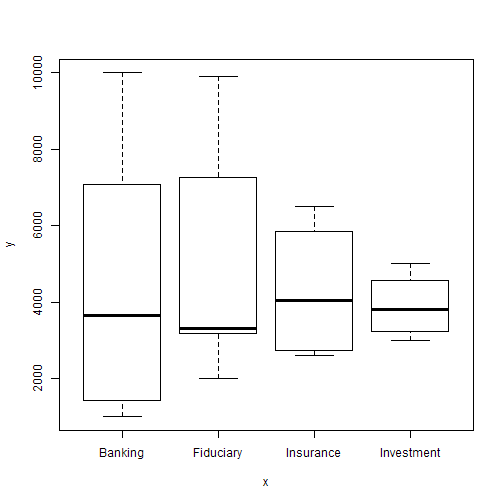
\includegraphics{r_training_data_analysis_presentation_files/figure-latex/plotting_example_1_hidden-1} \end{center}

\begin{center}\rule{0.5\linewidth}{\linethickness}\end{center}

\hypertarget{plotting---example-2}{%
\subsection{Plotting - example}\label{plotting---example-2}}

\begin{itemize}
\tightlist
\item
  As you can see, we've specified our x and y axis, but not what type of
  plot we want
\end{itemize}

--

\begin{itemize}
\tightlist
\item
  But the \texttt{plot()} function has guessed that we probably want a
  boxplot
\end{itemize}

--

\begin{itemize}
\tightlist
\item
  Note: you can also force R to create a boxplot using the
  \texttt{boxplot()} function
\end{itemize}

\begin{center}\rule{0.5\linewidth}{\linethickness}\end{center}

\hypertarget{plotting---example-3}{%
\subsection{Plotting - example}\label{plotting---example-3}}

\begin{itemize}
\tightlist
\item
  Next, we might want to see if there's a correlation between the income
  of a firm and the number of employees it has
\end{itemize}

--

\begin{itemize}
\tightlist
\item
  Again, we can use the plot function, specify our x and y axis, and R
  will guess what the best plot is
\end{itemize}

--

\begin{Shaded}
\begin{Highlighting}[]
\KeywordTok{plot}\NormalTok{(}\DataTypeTok{x =}\NormalTok{ test_data}\OperatorTok{$}\NormalTok{Income, }\DataTypeTok{y =}\NormalTok{ test_data}\OperatorTok{$}\NormalTok{Employees)}
\end{Highlighting}
\end{Shaded}

\begin{center}\rule{0.5\linewidth}{\linethickness}\end{center}

\hypertarget{plotting---example-4}{%
\subsection{Plotting - example}\label{plotting---example-4}}

\begin{center}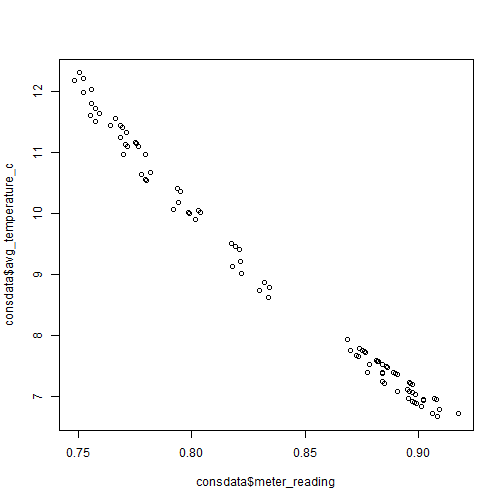
\includegraphics{r_training_data_analysis_presentation_files/figure-latex/plotting_example_2_hidden-1} \end{center}

\begin{center}\rule{0.5\linewidth}{\linethickness}\end{center}

\hypertarget{plotting---example-5}{%
\subsection{Plotting - example}\label{plotting---example-5}}

\begin{itemize}
\tightlist
\item
  R has created a scatter plot by default, but we can change the type if
  we wish using the option ``type'' argument
\item
  See your help sheet for the different types
\end{itemize}

\begin{center}\rule{0.5\linewidth}{\linethickness}\end{center}

\hypertarget{plotting---exercise}{%
\subsection{Plotting - exercise}\label{plotting---exercise}}

\begin{itemize}
\tightlist
\item
  Create a plot of employees against Lead Divisions\ldots{}
\end{itemize}

\begin{center}\rule{0.5\linewidth}{\linethickness}\end{center}

\hypertarget{plotting---answer}{%
\subsection{Plotting - answer}\label{plotting---answer}}

\begin{Shaded}
\begin{Highlighting}[]
\KeywordTok{plot}\NormalTok{(}\DataTypeTok{x =}\NormalTok{ test_data}\OperatorTok{$}\NormalTok{LeadDivision, }\DataTypeTok{y =}\NormalTok{ test_data}\OperatorTok{$}\NormalTok{Employees)}
\end{Highlighting}
\end{Shaded}

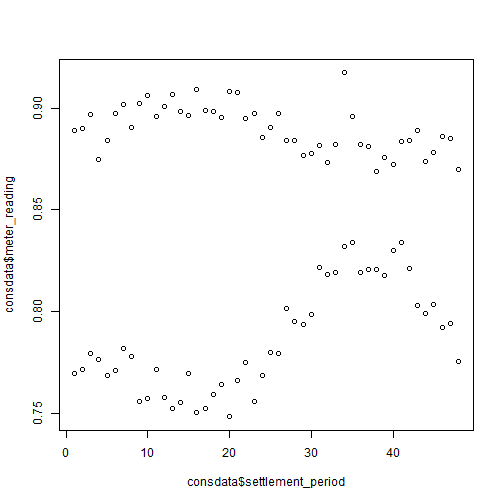
\includegraphics{r_training_data_analysis_presentation_files/figure-latex/plotting_exercise-1.pdf}

\begin{center}\rule{0.5\linewidth}{\linethickness}\end{center}

\hypertarget{histograms---example}{%
\subsection{Histograms - example}\label{histograms---example}}

\begin{itemize}
\tightlist
\item
  One of the best features of the plotting system in R is how easy it is
  to make histograms
\end{itemize}

--

\begin{itemize}
\tightlist
\item
  You can either use the \texttt{plot()} function and specify ``h'' as
  the type, or we can use the \texttt{hist()} function and provide one
  variable to produce a simple histogram\ldots{}
\end{itemize}

--

\begin{Shaded}
\begin{Highlighting}[]
\KeywordTok{hist}\NormalTok{(test_data}\OperatorTok{$}\NormalTok{Income)}
\end{Highlighting}
\end{Shaded}

\begin{center}\rule{0.5\linewidth}{\linethickness}\end{center}

\hypertarget{histograms---example-1}{%
\subsection{Histograms - example}\label{histograms---example-1}}

\begin{center}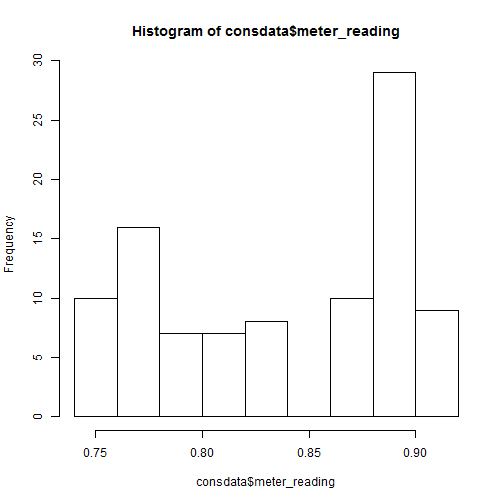
\includegraphics{r_training_data_analysis_presentation_files/figure-latex/histograms_hidden-1} \end{center}

\begin{center}\rule{0.5\linewidth}{\linethickness}\end{center}

\hypertarget{customizing-your-graphs}{%
\subsection{Customizing your graphs}\label{customizing-your-graphs}}

\begin{itemize}
\tightlist
\item
  To make your graph easier to understand, you may want to\ldots{}

  \begin{itemize}
  \tightlist
  \item
    Change the title
  \item
    Change the axis labels
  \item
    Change the points
  \item
    Change the size of the bins for our histogram
  \end{itemize}
\end{itemize}

--

\begin{itemize}
\tightlist
\item
  Note: These are a few of the customization options, but there are
  many, many more
\end{itemize}

\begin{center}\rule{0.5\linewidth}{\linethickness}\end{center}

\hypertarget{customizing-your-graphs-1}{%
\subsection{Customizing your graphs}\label{customizing-your-graphs-1}}

\begin{itemize}
\tightlist
\item
  Change the title

  \begin{itemize}
  \tightlist
  \item
    To change the title, all we need to do is specify a ``main''
    parameter in our plot function\ldots{}
  \end{itemize}
\end{itemize}

--

\begin{Shaded}
\begin{Highlighting}[]
\KeywordTok{plot}\NormalTok{(test_data}\OperatorTok{$}\NormalTok{Income, test_data}\OperatorTok{$}\NormalTok{Employees,}
     \DataTypeTok{main =} \StringTok{"Correlation between Income and # of Employees"}\NormalTok{)}
\end{Highlighting}
\end{Shaded}

--

\begin{itemize}
\tightlist
\item
  Change the axis labels

  \begin{itemize}
  \tightlist
  \item
    To change the labels on the axes, we use the ``xlab''/``ylab''"
    parameters\ldots{}
  \end{itemize}
\end{itemize}

--

\begin{Shaded}
\begin{Highlighting}[]
\KeywordTok{plot}\NormalTok{(test_data}\OperatorTok{$}\NormalTok{Income, test_data}\OperatorTok{$}\NormalTok{Employees,}
     \DataTypeTok{main =} \StringTok{"Correlation between Income and # of Employees"}\NormalTok{,}
     \DataTypeTok{xlab =} \StringTok{"Income (£)"}\NormalTok{,}
     \DataTypeTok{ylab =} \StringTok{"Number of Employees"}\NormalTok{)}
\end{Highlighting}
\end{Shaded}

\begin{center}\rule{0.5\linewidth}{\linethickness}\end{center}

\hypertarget{customizing-your-graphs-2}{%
\subsection{Customizing your graphs}\label{customizing-your-graphs-2}}

\begin{itemize}
\tightlist
\item
  Changing the graph points

  \begin{itemize}
  \tightlist
  \item
    To change the points, we use the ``pch'' paremeter, and specify a
    value between 0 and 25\ldots{}
  \end{itemize}
\end{itemize}

--

\begin{Shaded}
\begin{Highlighting}[]
\KeywordTok{plot}\NormalTok{(test_data}\OperatorTok{$}\NormalTok{Income, test_data}\OperatorTok{$}\NormalTok{Employees,}
     \DataTypeTok{main =} \StringTok{"Correlation between Income and # of Employees"}\NormalTok{,}
     \DataTypeTok{xlab =} \StringTok{"Income (£)"}\NormalTok{,}
     \DataTypeTok{ylab =} \StringTok{"Number of Employees"}\NormalTok{,}
     \DataTypeTok{pch =} \DecValTok{19}\NormalTok{)}
\end{Highlighting}
\end{Shaded}

\begin{itemize}
\tightlist
\item
  Putting those all together\ldots{}
\end{itemize}

\begin{center}\rule{0.5\linewidth}{\linethickness}\end{center}

\hypertarget{customizing-your-graphs-3}{%
\subsection{Customizing your graphs}\label{customizing-your-graphs-3}}

\begin{center}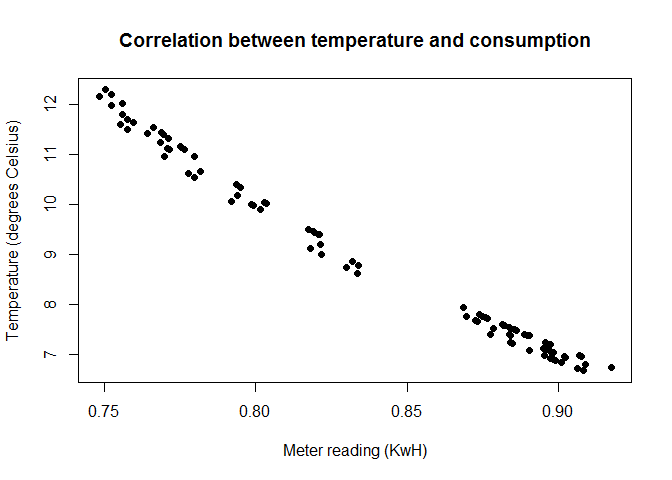
\includegraphics{r_training_data_analysis_presentation_files/figure-latex/customizing_graphs_total-1} \end{center}

\begin{center}\rule{0.5\linewidth}{\linethickness}\end{center}

\hypertarget{customizing-your-graphs-histograms}{%
\subsection{Customizing your graphs
(histograms)}\label{customizing-your-graphs-histograms}}

\begin{itemize}
\tightlist
\item
  In addition to the previous customization options, for histograms, we
  can change the size of the bins
\end{itemize}

--

\begin{itemize}
\tightlist
\item
  To do this, we specify the ``breaks'' parameter in our \texttt{hist()}
  function
\end{itemize}

--

\begin{itemize}
\tightlist
\item
  This splits up out our data into x number of bins of equal size
\end{itemize}

--

\begin{Shaded}
\begin{Highlighting}[]
\KeywordTok{hist}\NormalTok{(test_data}\OperatorTok{$}\NormalTok{Income, }\DataTypeTok{breaks =} \DecValTok{30}\NormalTok{)}
\end{Highlighting}
\end{Shaded}

\begin{center}\rule{0.5\linewidth}{\linethickness}\end{center}

\hypertarget{customizing-your-graphs-histograms-1}{%
\subsection{Customizing your graphs
(histograms)}\label{customizing-your-graphs-histograms-1}}

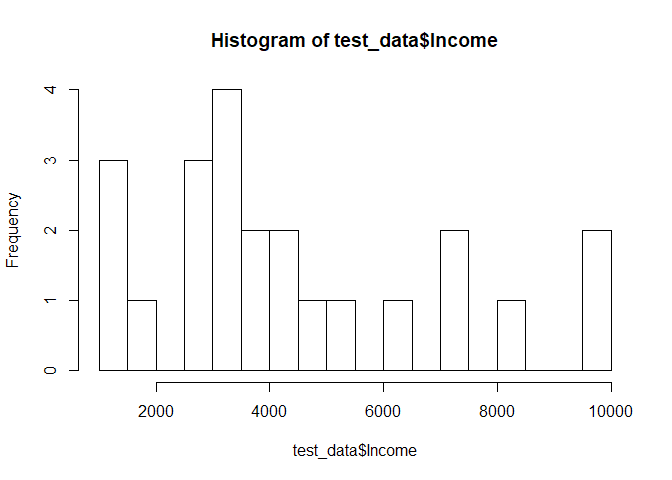
\includegraphics[width=0.5\linewidth]{r_training_data_analysis_presentation_files/figure-latex/customizing_graphs_hist_hidden-1}
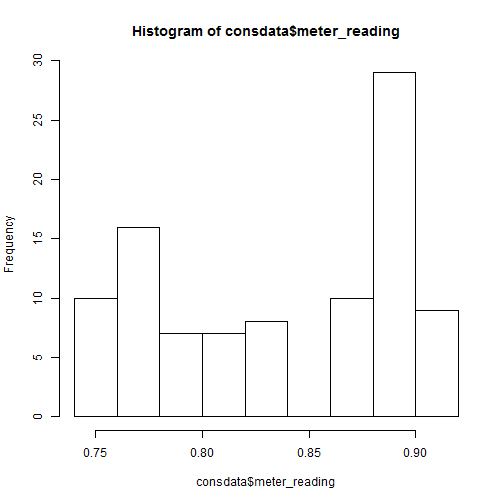
\includegraphics[width=0.5\linewidth]{r_training_data_analysis_presentation_files/figure-latex/customizing_graphs_hist_hidden-2}

\begin{center}\rule{0.5\linewidth}{\linethickness}\end{center}

\hypertarget{plotting---final-exercise}{%
\subsection{Plotting - final exercise}\label{plotting---final-exercise}}

\begin{itemize}
\tightlist
\item
  Create a plot of your choice, and change the title and axis labels.
\end{itemize}

\begin{center}\rule{0.5\linewidth}{\linethickness}\end{center}

\hypertarget{plotting---conclusion}{%
\subsection{Plotting - conclusion}\label{plotting---conclusion}}

\begin{itemize}
\tightlist
\item
  In short, R has lots of in-built tools to make quick, simple graphs
  and plots
\end{itemize}

--

\begin{itemize}
\tightlist
\item
  Most types of graph only require a few input parameters, but there's
  lots of customization options
\end{itemize}

--

\begin{itemize}
\tightlist
\item
  In a later module, we'll look at a package called ggplot2, which we'll
  use to create more complex graphics
\end{itemize}

\begin{center}\rule{0.5\linewidth}{\linethickness}\end{center}

\hypertarget{conclusion}{%
\subsection{Conclusion}\label{conclusion}}

\begin{itemize}
\tightlist
\item
  Installing packages

  \begin{itemize}
  \tightlist
  \item
    \texttt{install.packages()}, \texttt{library()}
  \end{itemize}
\item
  Loading data

  \begin{itemize}
  \tightlist
  \item
    \texttt{read.csv()}/\texttt{read.xlsx()}
  \end{itemize}
\item
  Cleaning data

  \begin{itemize}
  \tightlist
  \item
    Data type checks
  \item
    Data type conversion

    \begin{itemize}
    \tightlist
    \item
      Look out for dates and factors!
    \end{itemize}
  \end{itemize}
\item
  Plotting

  \begin{itemize}
  \tightlist
  \item
    \texttt{plot()}/\texttt{hist()}
  \end{itemize}
\item
  Customization

  \begin{itemize}
  \tightlist
  \item
    ``main'', ``xlab'', ``ylab'', ``pch'', ``breaks''
  \end{itemize}
\end{itemize}

\begin{center}\rule{0.5\linewidth}{\linethickness}\end{center}

\hypertarget{next-time}{%
\subsection{Next time\ldots{}}\label{next-time}}

\begin{itemize}
\tightlist
\item
  Creating functions
\item
  For loops
\item
  If else statements
\end{itemize}


\end{document}
